\section{MCU}
		The system will be microcontrolled rather than microprocessed because this is the most practical way to ensure that the real-time constrain will be respected. The choosen microcontroller is the \textit{ATmega328p} developed by \textit{Atmel Corporation} with 32 Kb of flash memory, 1 Kb of \textit{EEPROM} (Electrically Erasable Programmable Read-Only Memory), 32Kb of \textit{SRAM} (Static Random Access Memory) and a 16 MHz clock. This microncontroller is widely used in academic environment (specially after the Arduino project started, when microncontroller programming became much more feasible and reachable), and is famous for being easy and reliable to use. The \textit{ATmega328p} has six ADC inputs with a resolution of 10 bits and more 14 GPIO ports. This microcontroller also has serial communication, I$^2$C communication and other convinient features. It is really versatile and more important it meets this project requirements. The Figure \ref{fig-atmega328p} shows the pinage of this device in it's most commom footprint (DIP28).

		\begin{figure}[htbp]
			\centering
			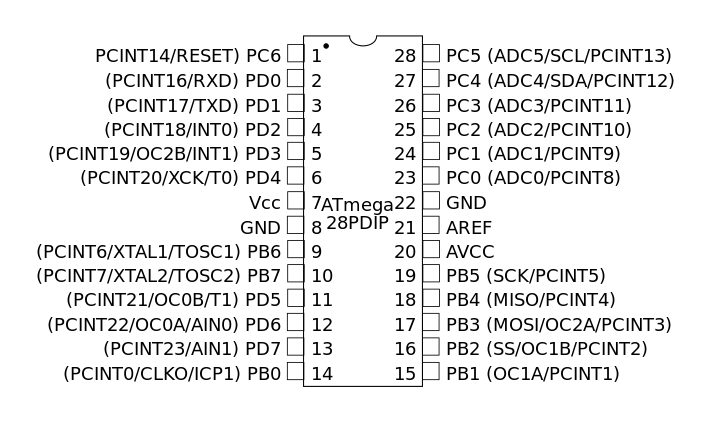
\includegraphics[scale=0.7]{figuras/fig-atmega328p.png}
			\caption{\textit{ATmega238p} \cite{coorporation2011atmel}}
			\label{fig-atmega328p}
		\end{figure}
	
